% use paper, or submit
% use 11 pt (preferred), 12 pt, or 10 pt only

\documentclass[letterpaper, paper,11pt]{AAS}	% for preprint proceedings
%\documentclass[letterpaper, paper,11pt]{AAS}		% for final proceedings (20-page limit)
%\documentclass[letterpaper, paper,12pt]{AAS}		% for final proceedings (20-page limit)
%\documentclass[letterpaper, paper,10pt]{AAS}		% for final proceedings (20-page limit)
%\documentclass[letterpaper, submit]{AAS}			% to submit to JAS

\usepackage{bm}
\usepackage{amsmath}
\usepackage{subcaption}
\usepackage{adjustbox}
\usepackage{algorithm}
\usepackage{algpseudocode}
%\usepackage{algpseudocode}
%\usepackage[notref,notcite]{showkeys}  % use this to temporarily show labels
\usepackage[colorlinks=true, pdfstartview=FitV, linkcolor=black, citecolor= black, urlcolor= black]{hyperref}
\usepackage{overcite}
\usepackage{footnpag}			      	% make footnote symbols restart on each page
\usepackage{enumitem}
\usepackage{booktabs}
\usepackage{slashbox}
\usepackage{multirow}
\usepackage{minted}
\raggedbottom


%\newcommand\scalemath[2]{\scalebox{#1}{\mbox{\ensuremath{\displaystyle #2}}}}
\NewDocumentCommand{\codeword}{v}{%
\texttt{\textcolor{black}{#1}}%
}

\PaperNumber{XX-XXX}



\begin{document}

\title{DRONE STATE ESTIMATION USING MULTIPLE INFRARED CAMERAS}

\author{Kadhir Umasankar\thanks{Graduate Student, Daniel Guggenheim School of Aerospace Engineering, kadhir.umasankar@gatech.edu}}


\maketitle{} 		


\begin{abstract}
% TODO: come back at the end
A motion capture system is generally used to estimate drone states in GPS-denied laboratory environments. For this setup, some reflective markers are attached to the drone, and multiple infrared cameras are positioned around the experiment area. The reflective markers' positions in space, along with their relative positions with respect to each other, are captured by the cameras, processed by software on the command center computer and are used to return the 3D position, velocities, and roll, pitch, and yaw of the drone. In this study, a system that uses multiple cameras (with their individual errors) will be simulated to estimate the state of the drone. This study proposes using a linear–quadratic regulator (LQR) controller, which will calculate the input needed to the drone at each timestep, allowing more trajectories to be analyzed. This is novel from past studies which assume constant inputs to the drone.
\end{abstract}


\section{Introduction}
%TODO add a lot of references while reading through
Drones generally use GPS measurements in conjunction with measurements from an IMU to estimate their position, velocity, and their roll, pitch, and yaw. In laboratory environments, the drones cannot use GPS data to complement other sensory inputs, so a motion capture system is usually used\cite{vicon_2022}. In such a system, a local origin is set, and the drone uses that as the origin of its inertial frame of reference.

One of the most common kinds of motion capture is optical-passive motion capture. The setup for this involves placing retro-reflective markers at various places on the drone, as can be seen in Figure~\ref{fig:MotionCaptureDrone}. Multiple infrared cameras are positioned around the experiment area, and they flash and capture infrared light reflected back from the retro-reflective markers at rates of more than 120 Hz. Such high input frequency is important when testing controllers, as a high sample rate would allow the controller to control better against sudden changes in the state of the system. Figure~\ref{fig:ViconMotionCaptureSpace} shows an example setup of a motion capture space.


\begin{figure}[htb]
\centering
\begin{subfigure}{.5\textwidth}
	\centering
	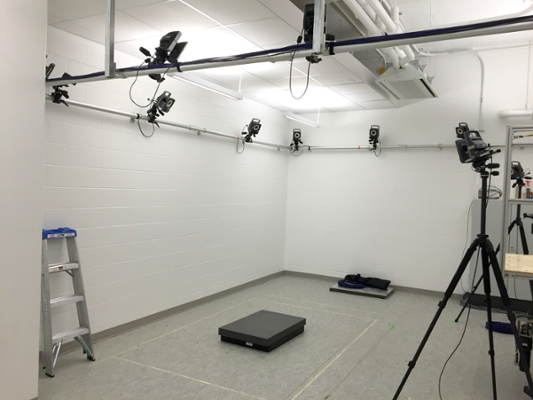
\includegraphics[width=0.9\textwidth]{Figures/ViconMotionCaptureSpace}
	\caption{Example motion capture space setup\cite{ViconMotionCaptureSpace}}
	\label{fig:ViconMotionCaptureSpace}
\end{subfigure}%
\begin{subfigure}{.5\textwidth}
	\centering
	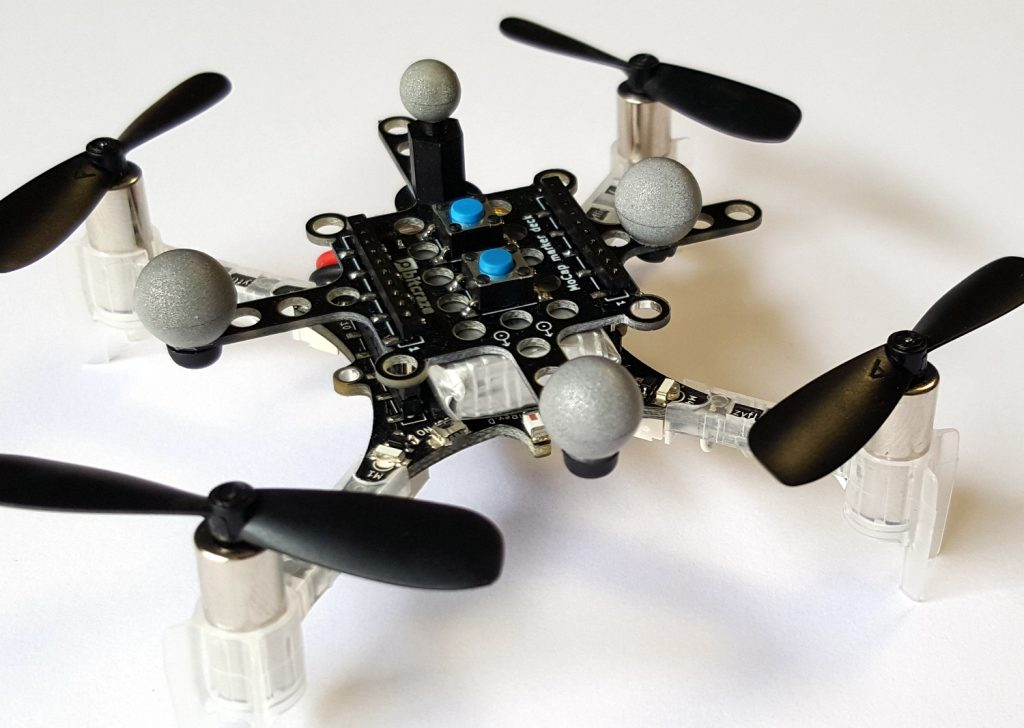
\includegraphics[width=0.9\textwidth]{Figures/MotionCaptureDrone}
	\caption{Example drone with retro-reflective markers\cite{MotionCaptureDrone}}
	\label{fig:MotionCaptureDrone}
\end{subfigure}
\caption{Example setup that could be used if this study were to be repeated on real-life data}
\label{fig:MotionCaptureExample}
\end{figure}

Most previous studies in drone state estimation have assumed constant inputs\cite{Study, Study2}. In this study, a linear-quadratic regulator (LQR) controller will be used to find the inputs to the system's dynamics at every timestep, thereby allowing more types of flight paths to be tracked. This study will use simulated motion capture system data to estimate the states of a drone in various flight patterns. The simulation will take place in a Gazebo 3D simulation environment\cite{gazebo}. A ROS (Robot Operating System)\cite{ros} package will be used to perform control and trajectory planning for the drone, and logs of the flight data will be run through an Extended Kalman filter (EKF) and an Unscented Kalman filter (UKF) in MATLAB to obtain an accurate estimate of the state of the drone. A Kalman filter is vital for drone state estimation, as sensors generally create a lot of noise, and the filter will account for the noise and provide a more accurate estimate of the output\cite{Alejandro}. The performance of the filters on flight paths of varying levels of difficulty will be analyzed.

% TODO: The remainder of the paper is organized as follows.

% TODO: come up with better names later
\section{Simulation Setup}

Data for this study was obtained through simulation. The drone chosen for this experiment was the 3DR Iris\cite{iris}, a model of which is available for use in Gazebo\cite{gazebo}. The Spatial Data File (SDF) of the Iris' model was edited to include four reflective markers. The positions of these markers can be seen in Table~\ref{tab:DroneModel} and Figure~\ref{fig:DroneModel}. This drone also contains an IMU, and the Spatial Data File of the Iris' model showed that it is located at the centroid of the drone.

\begin{table}[htbp]
	\fontsize{10}{10}\selectfont
    \caption{Positions of the reflective markers (in cm) with respect to the centroid of the drone}
   \label{tab:DroneModel}
        \centering 
   \begin{tabular}{c | c | c | c} % Column formatting, 
      \hline 
      Marker Number    & x & y & z \\
      \hline 
      1      & 10.5 & 0 & 0 \\
      2      & 0 & 6.0 & 0 \\
      3      & -11.5 & 0 & 0 \\
      4      & 0 & -6.0 & 0 \\
      \hline
   \end{tabular}
\end{table}

\begin{figure}[htb]
	\centering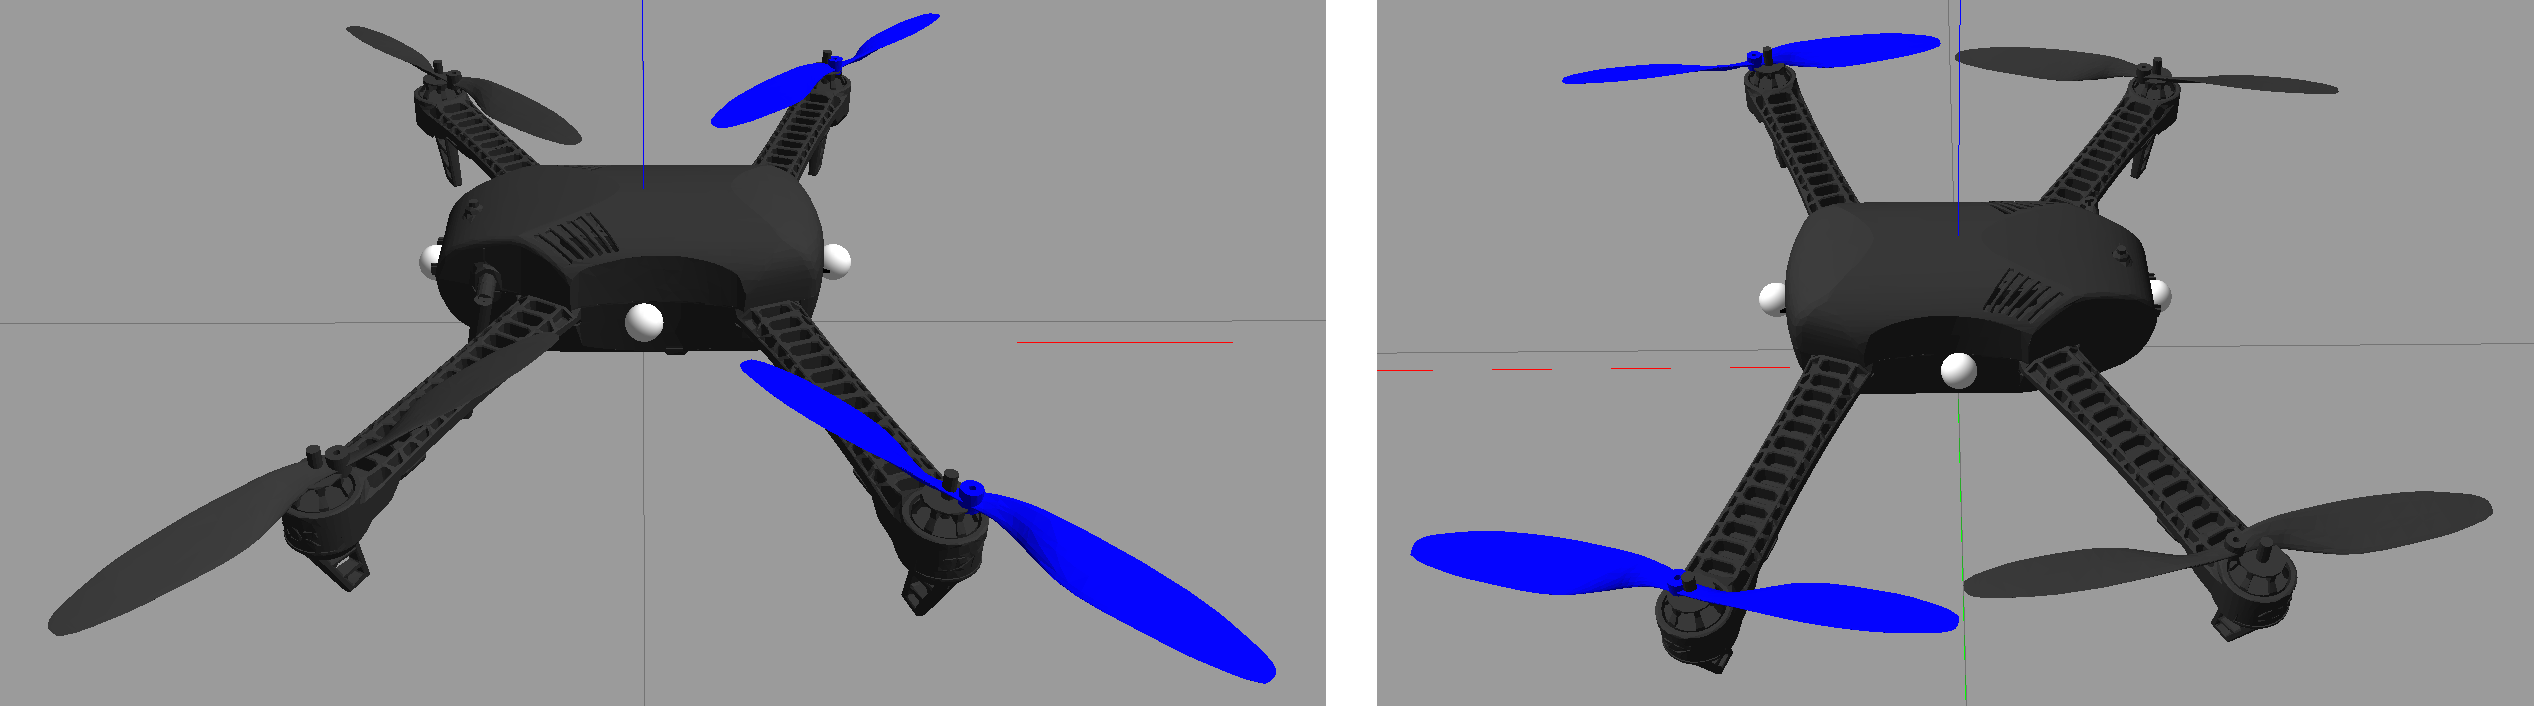
\includegraphics[width=5in]{Figures/DroneModel}
	\caption{Side views of the drone that will be used for simulation}
	\label{fig:DroneModel}
\end{figure}

%TODO add more citations

A world with four Vicon Vantage V16 infrared cameras was then created in Gazebo, and their coordinates can be seen in Table~\ref{tab:cameras}. Figure~\ref{fig:GazeboWorld} shows the setup of the environment. The distance from these cameras to reflective markers on the drone was measured at a rate of approximately 120 Hz, which is consistent with the spec sheet of the Vicon Vantage V16\cite{V16}.

\begin{table}[htbp]
	\fontsize{10}{10}\selectfont
    \caption{Coordinates of the cameras in meters}
   \label{tab:cameras}
        \centering 
   \begin{tabular}{c | c | c | c} % Column formatting, 
      \hline 
      Camera ID    & x & y & z \\
      \hline 
      1      & 10 & 10 & 10 \\
      2      & -10 & 10 & 10 \\
      3      & -10 & -10 & 10 \\
      4      & 10 & -10 & 10 \\
      \hline
   \end{tabular}
\end{table}

\begin{figure}[htb]
	\centering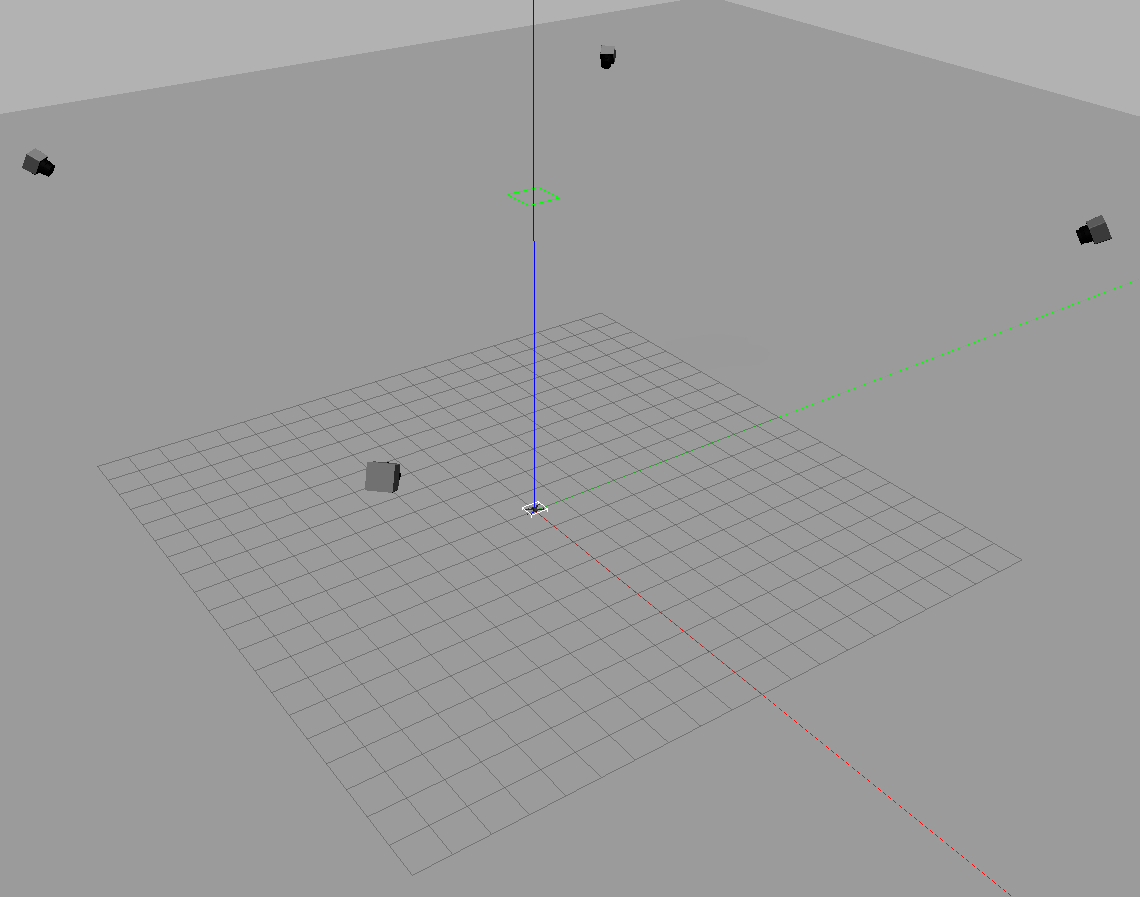
\includegraphics[width=3in]{Figures/GazeboWorld}
	\caption{The Gazebo world that the simulation will take place in. Each square has a side length of 1 m. Thus, the entire world is 10m $\times$ 10 m $\times$ 10 m. Cameras can be seen positioned at coordinates consistent with Table~\ref{tab:cameras}}
	\label{fig:GazeboWorld}
\end{figure}

A ROS package was used to control the drone in simulation. The measurements were recorded to ROSbags (the file format used by ROS to store message data), and will later be analyzed in MATLAB.

\section{Dynamics Modeling}

Eq.~\eqref{eq:X} shows the state vector, where $x$, $y$, and $z$ are the $x$, $y$, and $z$ positions of the drone, $v_x$, $v_y$, and $v_z$ are the $x$, $y$, and $z$ velocities of the drone, $\phi$, $\theta$, and $\psi$ are the roll, pitch, and yaw of the drone, and $p$, $q$, and $r$ are the body angular velocities in terms of Euler angles and Euler rates. 
\setcounter{MaxMatrixCols}{12}
\begin{equation}
	\label{eq:X}
	X = \begin{bmatrix}
		x & y & z & v_x & v_y & v_z & \phi & \theta & \psi & p & q & r
\end{bmatrix}^T
\end{equation}

Taking the time derivative of $X_1$ through $X_3$ from Eq. \eqref{eq:X} gives Eq. \eqref{eq:X1dot}.

\begin{equation}
\begin{bmatrix}
\dot{x}\\
\dot{y}\\
\dot{z}
\end{bmatrix} =
\begin{bmatrix}
v_x \\
v_y\\
v_z
\end{bmatrix}
\label{eq:X1dot}
\end{equation}

The drone's velocity (i.e. $v_x$, $v_y$, $v_z$) will be perturbed by thrust on the drone. However, the thrust will only act in the positive $z$-direction of the drone body-fixed frame, denoted by $Z_b$ in Figure~\ref{fig:DroneFrame}. Thus, the thrust input must be rotated with respected to the roll, pitch, and yaw of the drone to find its effect along the $X_i$, $Y_i$, and $Z_i$ directions. An Euler 123 rotation, denoted by $R_{123}$ in Eq.~\eqref{eq:R} is used to rotate from the body frame to the inertial frame\footnote{Throughout this report, $c$, $s$, and $t$ will be used in place of $\cos$, $\sin$, and $\tan$ for brevity}. Combining these steps, taking the time derivative of $X_4$ through $X_6$ gives Eq. \eqref{eq:X2dot}.

\begin{figure}[htb]
	\centering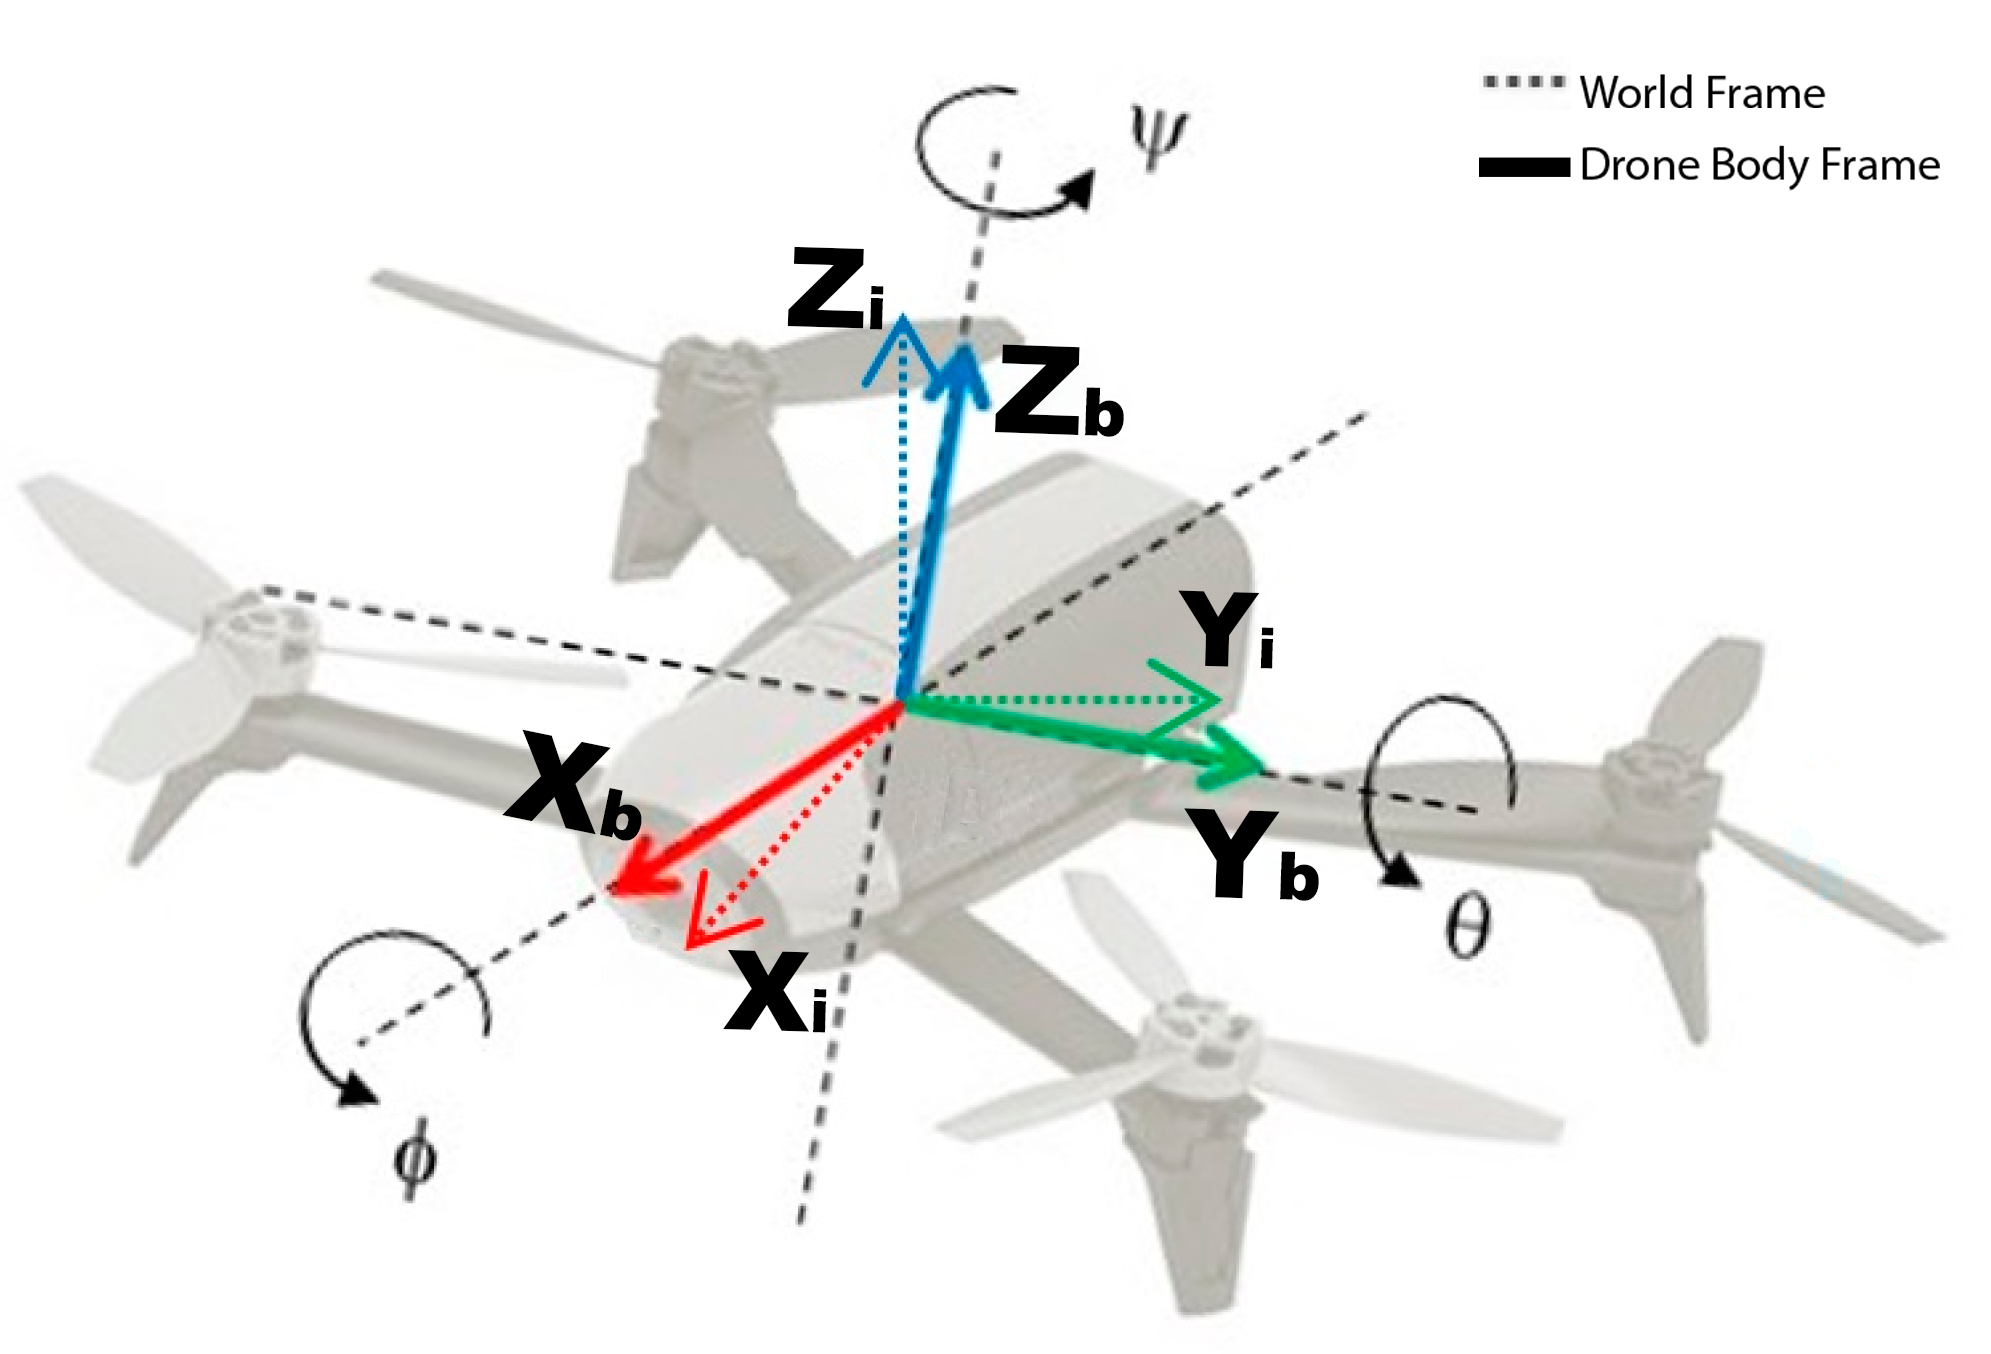
\includegraphics[width=0.5\textwidth]{Figures/DroneFrame}
	\caption{An illustration comparing the inertial world frame (denoted by dotted lines), and the body-fixed frame (denoted by solid lines)}\cite{DroneFrame}
	\label{fig:DroneFrame}
\end{figure}

\begin{equation}
\label{eq:R}
\begin{split}
R_{123} &= R_z(\psi)R_y(\theta)R_x(\phi) = \begin{bmatrix}
c(\psi) & s(\psi) & 0 \\
s(\psi) & c(\psi) & 0 \\
0 & 0 & 1
\end{bmatrix}
\begin{bmatrix}
c(\theta) & 0 & s(\theta) \\
0 & 1 & 0 \\
-s(\theta) & 0 & c(\theta)
\end{bmatrix}
\begin{bmatrix}
1&0&0\\
0&c(\phi)&-s(\phi)\\
0&s(\phi)&c(\phi)
\end{bmatrix}\\
&=
\begin{bmatrix}
c(\theta)c(\psi) & c(\psi)s(\theta)s(\phi) - c(\phi)s(\psi) & s(\phi)s(\psi) + c(\phi)c(\psi)s(\theta) \\
c(\theta)s(\psi) & c(\phi)c(\psi) + s(\theta)s(\phi)s(\psi) & c(\phi)s(\theta)s(\psi) - c(\psi)s(\phi) \\
-s(\theta) & c(\theta)s(\phi) & c(\theta)c(\phi) 
\end{bmatrix}
\end{split}
\end{equation}

\begin{equation}
\label{eq:X2dot}
\begin{bmatrix}
\dot{v}_x\\
\dot{v}_y\\
\dot{v}_z\\
\end{bmatrix}
= \frac{R_{123}
\begin{bmatrix}
0\\
0\\
u_3
\end{bmatrix}
-
\begin{bmatrix}
0\\
0\\
mg
\end{bmatrix}}{m}=
\begin{bmatrix}
(u_3(s(\phi)s(\psi) + c(\phi)c(\psi)s(\theta)))/m \\
-(u_3(c(\psi)s(\phi) - c(\phi)s(\theta)s(\psi)))/m \\
-(mg - u_3c(\theta)c(\phi))/m
\end{bmatrix}
\end{equation}

Similarly, $p$, $q$, and $r$ (i.e. the roll, pitch, and yaw rates) must be rotated into the body frame to find their effect on the roll, pitch, and yaw of the drone. Taking the time derivative of $X_7$ through $X_9$ then gives Eq.~\eqref{eq:X3dot}, which shows the rotation matrix used to rotate to the body frame.

\begin{equation}
\label{eq:X3dot}
\begin{bmatrix}
\dot{\phi}\\
\dot{\theta}\\
\dot{\psi}
\end{bmatrix}=
\begin{bmatrix}
1& s(\phi)t(\theta)&  c(\phi)t(\theta)\\
0& c(\phi)&          -s(\phi)\\
0& s(\phi)/c(\theta)&c(\phi)/c(\theta)
\end{bmatrix}
\begin{bmatrix}
p\\
q\\
r
\end{bmatrix}=
\begin{bmatrix}
p + r\cos(\phi)\tan(\theta) + q\tan(\theta)\sin(\phi) \\
q\cos(\phi) - r\sin(\phi) \\
(r\cos(\phi))/\cos(\theta) + (q\sin(\phi))/\cos(\theta)
\end{bmatrix}
\end{equation}

To find the change in $p$, $q$, and $r$, the rotational equations of motion can be derived from Euler’s equations for rigid body dynamics. Expressed in vector form, Euler’s equations are written as

\[
I\dot{\omega}+\omega\times(I\omega)=\tau
\]

where $\omega$ is the vector of angular rates $p$, $q$, and $r$, $I$ is the inertia matrix, and $\tau$ is a vector of the roll, pitch, and yaw torques. This can be rewritten as
% COMBAK: look at this
\[
\dot{\omega}=\begin{bmatrix}
\dot{p}\\
\dot{q}\\
\dot{r}\\
\end{bmatrix}=
I^{-1}\left(\begin{bmatrix}
u_4\\u_5\\u_6
\end{bmatrix}-
\begin{bmatrix}
p\\
q\\
r
\end{bmatrix}\times	I\begin{bmatrix}
p\\
q\\
r
\end{bmatrix}\right)
\]

where $u_4$ through $u_6$ are the roll, pitch, yaw torques on the drone respectively. To find the inertia matrix to be used in the previous equation, the quadcopter can be modeled as two thin uniform rods crossed at the origin with a point mass (the motor) at the end of each. This results in a diagonal inertia matrix of the form

\[
I = \begin{bmatrix}
I_{xx}&0&0\\
0&I_{yy}&0\\
0&0&I_{zz}
\end{bmatrix}
\]

Combining these steps, the final result of the time derivative of states $X_{10}$ through $X_{12}$ can be seen in Eq. \eqref{eq:X4dot} (Reference \cite{X4dot}).

\begin{equation}
\label{eq:X4dot}
\begin{bmatrix}
\dot{p}\\
\dot{q}\\
\dot{r}
\end{bmatrix}=
\begin{bmatrix}
(u_4 + I_{yy}qr - I_{zz}qr)/I_{xx}\\
(u_5 - I_{xx}pr + I_{zz}pr)/I_{yy}\\
(u_6 + I_{xx}qp - I_{yy}qp)/I_{zz}
\end{bmatrix}
\end{equation}

% COMBAK: DELETE THIS LATER!!!!!!!!
Combining Equations~\ref{eq:X1dot},~\ref{eq:X2dot},~\ref{eq:X3dot} and~\ref{eq:X4dot} gives Eq. \eqref{eq:Xdot} for $F$.


\begin{equation}
\label{eq:Xdot}
\dot{X}(t) = F(X(t), t) = \begin{bmatrix}
\dot{x} \\ \dot{y} \\ \dot{z} \\ \dot{v_x} \\ \dot{v_y} \\ \dot{v_z} \\ \dot{\phi} \\ \dot{\theta} \\ \dot{\psi} \\ \dot{p} \\ \dot{q} \\ \dot{r} 
\end{bmatrix} =  \begin{bmatrix}
v_x \\
v_y \\
v_z \\
(u_3(\sin(\phi)\sin(\psi) + \cos(\phi)\cos(\psi)\sin(\theta))/m \\
(-u_3(\cos(\psi)\sin(\phi) + \cos(\phi)\sin(\theta)\sin(\psi))/m \\
(u_3\cos(\theta)\cos(\phi) - mg)/m \\
p + r\cos(\phi)\tan(\theta) + q\tan(\theta)\sin(\phi) \\
q\cos(\phi) - r\sin(\phi) \\
\frac{r\cos(\phi)}{\cos(\theta)} + \frac{q\sin(\phi)}{\cos(\theta)} \\
\frac{u_4 + qrI_{yy} - qrI_{zz}}{I_{xx}} \\
\frac{u_5 - prI_{xx} + prI_{zz}}{I_{yy}} \\
\frac{u_6 + qpI_{xx} - qpI_{yy}}{I_{zz}} \\
\end{bmatrix}
\end{equation}

Taking the partial of $F$ with respect to $X$ gives $A$ in Eq. \eqref{eq:A}.
\begin{equation}
\label{eq:A}
A = \frac{\partial F}{\partial X} = 
\begin{bmatrix} 
    \frac{\partial F_1}{\partial x} & \dots  & \frac{\partial F_1}{\partial r}\\
    \vdots & \ddots & \vdots\\
    \frac{\partial F_{12}}{\partial x} & \dots  & \frac{\partial F_{12}}{\partial r} 
\end{bmatrix}
\end{equation}

\begin{figure}[H]
	\centering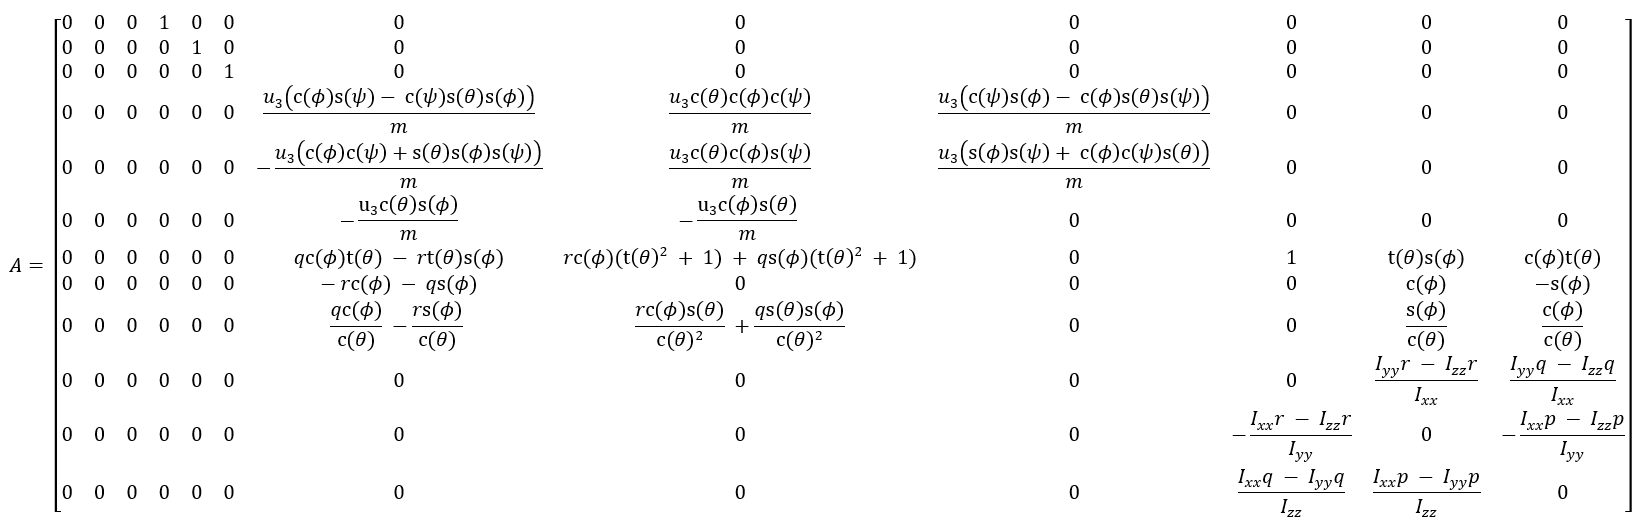
\includegraphics[width=\textwidth]{Figures/AMatrix}
	\caption{The final A matrix, where $c$, $s$, and $t$, are $\cos$, $\sin$, and $\tan$. (This was included as a figure since \LaTeX\ did not allow matrices this wide)}
	\label{fig:AMatrix}
\end{figure}

A model's Spatial Data file specifies its physical properties to be used by the simulator, so the drone's mass and moment of inertia values were taken from the file to be $m = 1.545\ \text{kg}$, $I_{xx} = 0.029125\ \text{kg}\cdot \text{m}^2$, $I_{yy} = 0.029125\ \text{kg}\cdot \text{m}^2$, and $I_{zz} = 0.055225\ \text{kg}\cdot \text{m}^2$, and $g = 9.81\ \text{m}/\text{s}^2$ was used.
It can be noticed from Eq.~\ref{eq:Xdot} that to propagate the drone's state forward, it is necessary to have some knowledge of the inputs to the system, $u_3$ through $u_6$, i.e. the thrust, and roll, pitch, yaw torques. A linear–quadratic regulator (LQR) controller will be created for this purpose. The LQR controller will take in the drone's current state, compute $A$ using Eq.~\ref{eq:A} with $u_3 = mg$, compute $B$ using Eq.~\ref{eq:B} (which takes the partial of F with respect to the inputs), and will use $Q$ and $R$ from Eq.~\ref{eq:QandR} to compute the optimal gain matrix for the LQR controller, $K$, such that $u=-Kx$ minimizes $J(u)=\int_{0}^{\infty} (x^TQx+u^TRu)dt$ subject to the system dynamics $\dot{x}=Ax+Bu$ (LQR logic further explained in Reference~\citenum{LQRBook}). The controller will return a vector of inputs $u_3$ through $u_6$ to control the drone\footnote{Note that $Q$, $R$, and $K$ in the LQR controller play a similar role as they do in the Kalman filter, but they are not the same value. The best values for $Q$ and $R$ were found by tuning them experimentally}. The LQR logic will be carried out using MATLAB's \texttt{lqr} function\cite{LQR}.

\begin{equation}
\begin{split}
\label{eq:B}
B &= \frac{\partial F}{\partial u} = 
\begin{bmatrix} 
    \frac{\partial F_1}{\partial u_3} & \dots  & \frac{\partial F_1}{\partial u_6}\\
    \vdots & \ddots & \vdots\\
    \frac{\partial F_{12}}{\partial u_3} & \dots  & \frac{\partial F_{12}}{\partial u_6} 
\end{bmatrix}\\&=\begin{bmatrix}
         0&0&0&0\\
         0&0&0&0\\
         0&0&0&0\\
         (\sin(\phi)\sin(\psi) + \cos(\phi)\cos(\psi)\sin(\theta)) / m&0&0&0\\
         -(\cos(\psi)\sin(\phi) - \cos(\phi)\sin(\theta)\sin(\psi)) / m&0&0&0\\
         (\cos(\phi)\cos(\theta)) / m&0&0&0\\
         0&0&0&0\\
         0&0&0&0\\
         0&0&0&0\\
         0&I_{xx}^{-1}&0&0\\
         0&0&I_{yy}^{-1}&0\\
         0&0&0&I_{zz}^{-1}
\end{bmatrix}
\end{split}
\end{equation}

\begin{equation}
\label{eq:QandR}
\begin{split}
Q &= \texttt{diag([100 100 100 100 100 100 0.1 0.1 0.1 10 10 10])}\\
R &= \texttt{diag([0.1 1000 1000 1000])}
\end{split}
\end{equation}

\section{Measurement Model}

The distance from the camera to the centroid of the drone was measured by each of the infrared cameras, and roll, pitch, yaw measurements of the drone would directly be measured using the IMU. To find the distance from the cameras to the centroid, the cameras would return the average distance of all of the reflective markers on the drone, which is roughly equal to the distance to the drone's centroid due to the way reflective markers were positioned on the drone. This math is done implicitly within the Vicon computer software, and just the ranges are returned. Thus, instead of maintaining a separate state for each reflective marker on the drone, it will be assumed that the measurement model uses the coordinates of the centroid to measure the range to the centroid\footnote{The alternative to this is to maintain the state of each marker separately, and propagate each state forward individually. However, since the reflective markers are placed almost symmetrically across the axes of the drone-fixed frame, this will offer little to no improvement in the accuracy of the estimates, and that possible slight improvement in accuracy will not outweigh the increase in computational time}. The roll, pitch, and yaw measurements will be used directly from the IMU measurements. The measurement model was then formulated as $G$ in Eq.~\ref{eq:G}, where $X_n$, $Y_n$, and $Z_n$ are the $X$, $Y$, and $Z$ coordinates of the $n$th camera in the global reference frame.

\begin{equation}
\label{eq:G}
G(X(t), t) = 
\begin{bmatrix}
	\sqrt{(x-X_1)^2 + (y-Y_1)^2 + (z-Z_1)^2} \\
	\sqrt{(x-X_2)^2 + (y-Y_2)^2 + (z-Z_2)^2} \\
	\sqrt{(x-X_3)^2 + (y-Y_3)^2 + (z-Z_3)^2} \\
	\sqrt{(x-X_4)^2 + (y-Y_4)^2 + (z-Z_4)^2} \\
	\phi \\
	\theta \\
	\psi
\end{bmatrix}
\end{equation}

% WHY DO WE FIND H, G y confuse panni solrene

The observation matrix, $H$, was found by taking the partial of the measurement model, $G$, with respect to $X$.

\begin{equation}
\label{eq:H}
H = \frac{\partial G}{\partial X} =
\begin{bmatrix} 
    \frac{\partial G_1}{\partial x} & \dots  & \frac{\partial G_1}{\partial r}\\
    \vdots & \ddots & \vdots\\
    \frac{\partial G_{7}}{\partial x} & \dots  & \frac{\partial G_{7}}{\partial r}
\end{bmatrix} 
\end{equation}

\begin{figure}[H]
	\centering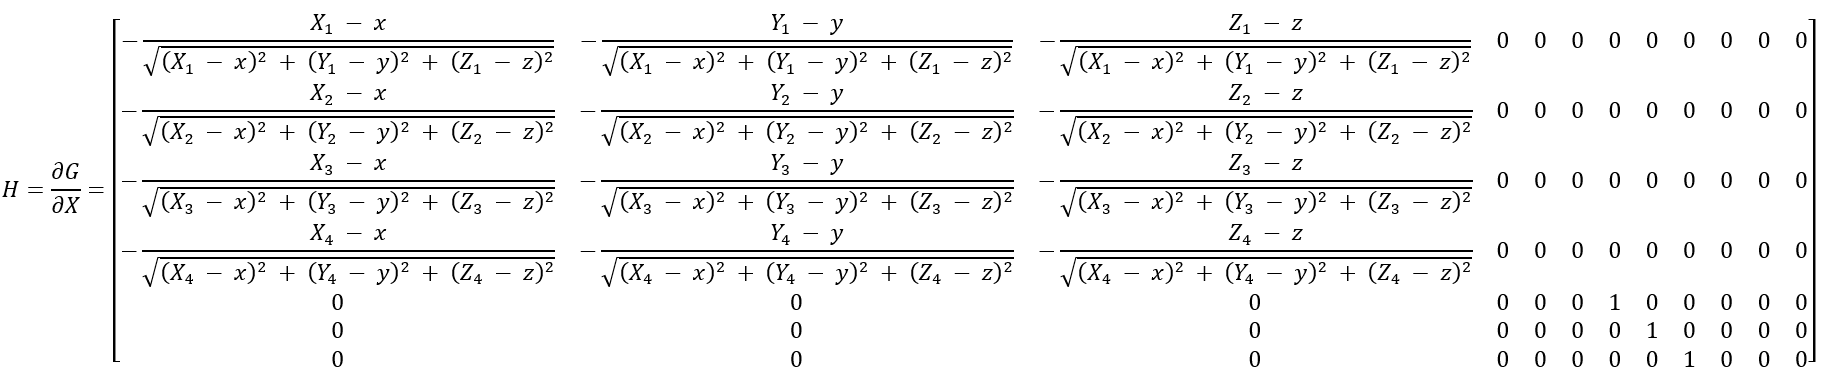
\includegraphics[width=\textwidth]{Figures/HMatrix}
	\caption{The final H matrix, where $X_n$, $Y_n$, and $Z_n$ are the $X$, $Y$, and $Z$ coordinates of the $n$th camera (This was included as a figure since \LaTeX\ did not allow matrices this wide)}
	\label{fig:HMatrix}
\end{figure}

\section{Filter Setup}
% TODO: maybe put the P and R info here

Using the aforementioned dynamics and measurement model, a hybrid Extended Kalman filter and an Unscented Kalman filter were implemented\cite{Simon}. The algorithms for these filters can be seen in Appendix A. The noise for the roll, pitch, yaw measurements was experimentally determined as $3.8785\cdot 10^{-5}$ radians of error along each axis by finding the variance of the IMU measurements when the drone was stationary. The noise for the range measurements was initially set to $1.5$ mm as per the claimed accuracy on the specsheet of the Vicon Vantage V16\cite{V16}. However, such small variances did not show how robust the filters were to non-ideal conditions. Hence, the variance of each of the four cameras was set to $0.0015^2$ m, $0.015^2$ m, $0.002^2$ m, and $0.1^2$ m to showcase the filters' robustness, and the aforementioned $3.8785\cdot 10^{-5}$ radians of error was used for the IMU measurements. Hence, the covariance matrix of the measurements was set to \codeword{R = diag([0.0015^2 0.015^2 0.002^2 0.1^2 (3.8785e-5)^2 (3.8785e-5)^2 (3.8785e-5)^2])}.

The a priori state covariance, $P_0^+$ was set to \codeword{diag([(0.001)^2 (0.001)^2 (0.001)^2 0 0 0 (3.8785e-5)^2 (3.8785e-5)^2 (3.8785e-5)^2 0 0 0])}, since it is possible that there were errors on the scale of millimeters when measuring the starting position of the drone, $3.8785\cdot 10^{-5}$ radians of error from the IMU measurements, and 0 error in the velocities and angular rates since it was at rest. For the Unscented Kalman Filter, the velocity and $p$, $q$, $r$ covariances were set as \codeword{(0.001)^2} and \codeword{(3.8785e-5)^2} respectively, since the $P_0^+$ matrix must be positive definite.

The code for this study can be found at \url{github.com}.
%TODO

\section{Experimental Procedure}

The range measurements from the cameras and the roll, pitch, yaw measurements from the IMU were stored as ROSbags, and were read into MATLAB. Four types of trajectories were used to analyze the performance of the filters for this study:
\begin{enumerate}[label=(\alph*)]
\item Hover - The drone hovers to a height of 3 m and lands (as seen in Figure~\ref{fig:hover1_just_traj})
\item Circle - The drone hovers to a height of 3 m and starts flying in a circle with radius 1 m (as seen in Figure~\ref{fig:circle1_just_traj})
\item Sine - The drone hovers to a height of 3 m and flies in a sine wave in the +x-direction (as seen in Figure~\ref{fig:sine1_just_traj})
\item Square - The drone hovers to a height of 3 m and flies in a square with a sidelength of 4 m (as seen in Figure~\ref{fig:square1_just_traj})
\end{enumerate}

The default sampling rate of the cameras was at 120 Hz, but the stored data was modified to replicate a measurement rate of 60 Hz, 24 Hz, 12 Hz, 6 Hz, and an extreme of 1 Hz, to determine how the filters performed with a scarcity of samples, and the performance of the filters over these measurement rates was compared.

% TODO: change the size of this later
\begin{figure}[H]
\centering
\begin{subfigure}{.4\textwidth}
	\centering
	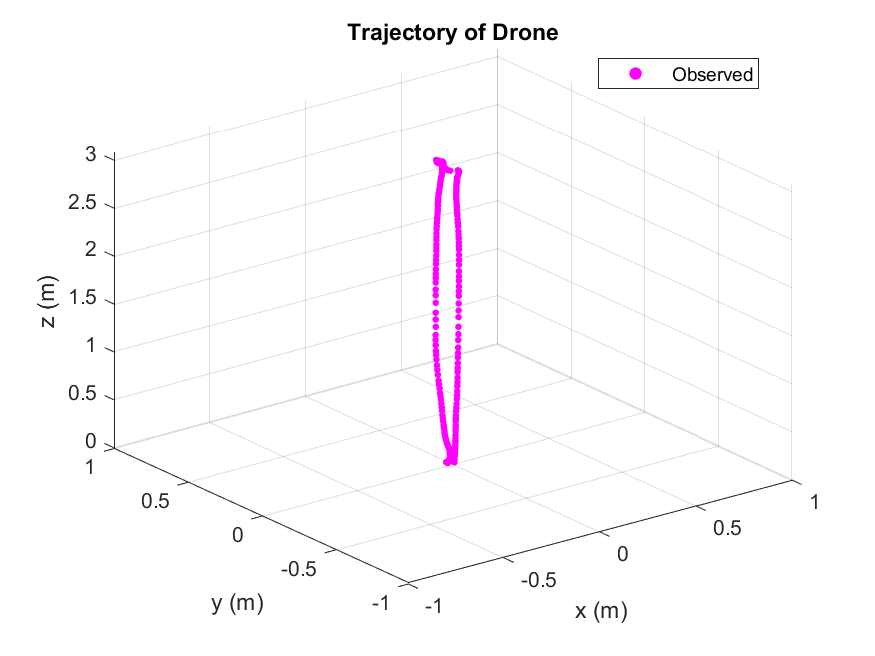
\includegraphics[width=0.9\textwidth]{Figures/hover1_just_traj}
	\caption{Hover trajectory}
	\label{fig:hover1_just_traj}
\end{subfigure}%
\begin{subfigure}{.4\textwidth}
	\centering
	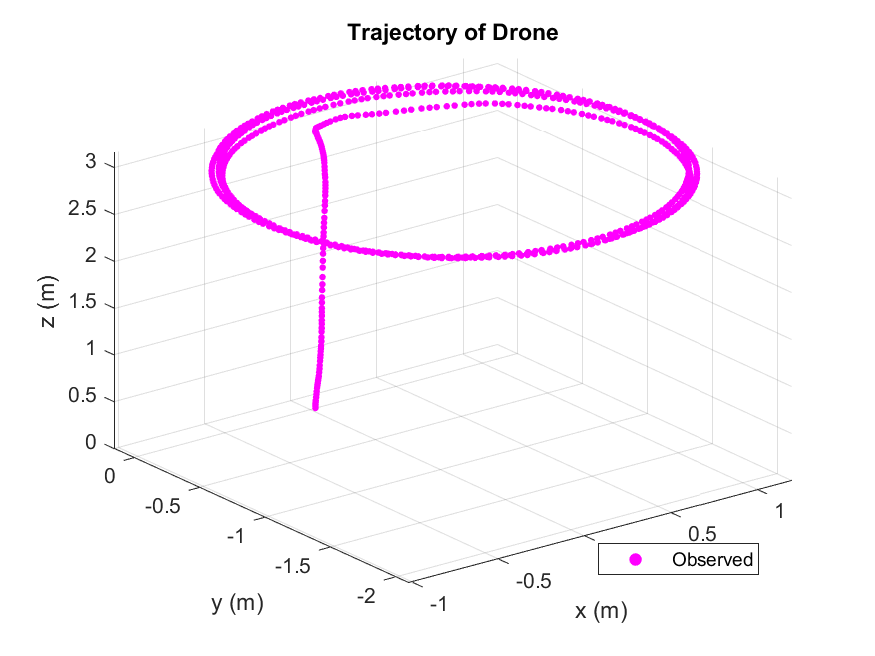
\includegraphics[width=0.9\textwidth]{Figures/circle1_just_traj}
	\caption{Circle trajectory}
	\label{fig:circle1_just_traj}
\end{subfigure}
\begin{subfigure}{.4\textwidth}
	\centering
	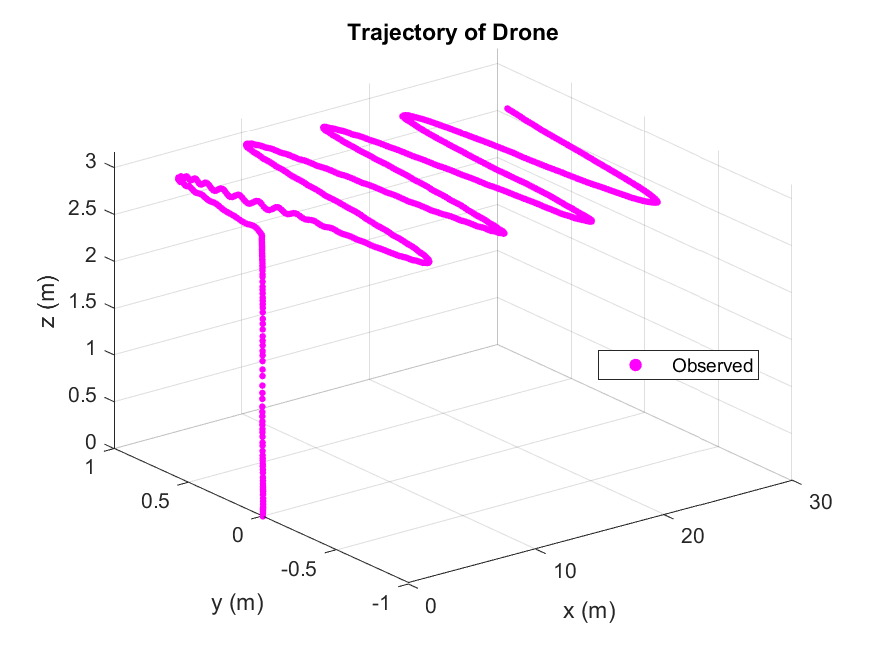
\includegraphics[width=0.9\textwidth]{Figures/sine1_just_traj}
	\caption{Sine trajectory}
	\label{fig:sine1_just_traj}
\end{subfigure}%
\begin{subfigure}{.4\textwidth}
	\centering
	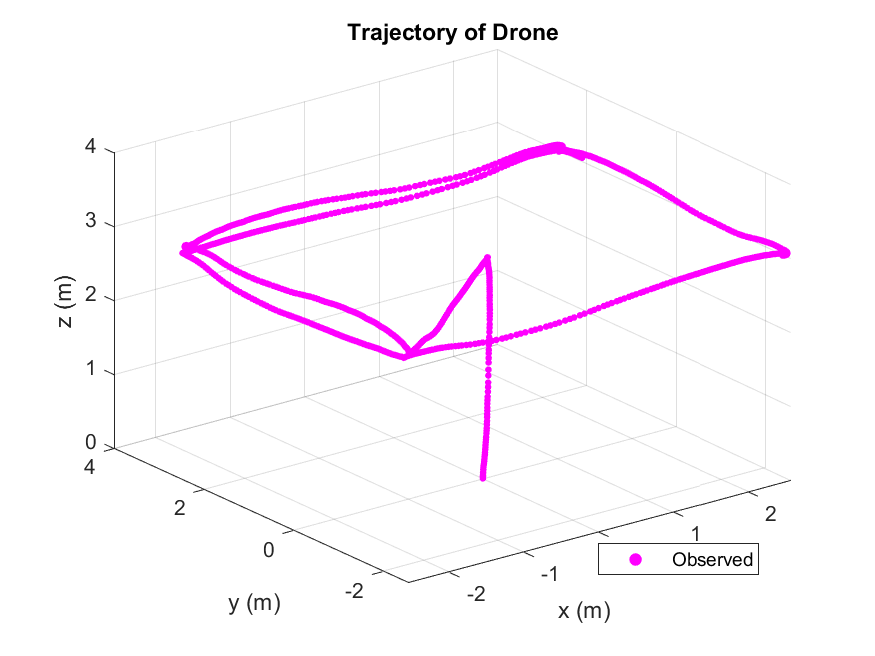
\includegraphics[width=0.9\textwidth]{Figures/square1_just_traj}
	\caption{Square trajectory}
	\label{fig:square1_just_traj}
\end{subfigure}
\caption{The trajectories that the drone followed}
\label{fig:DroneTrajectories}
\end{figure}

\section{Results and Discussion}

The results of the hybrid Extended Kalman filter will be discussed first. The EKF estimates can be seen overlayed on top of the observations in Figures~\ref{fig:Overlay1} and \ref{fig:Overlay2}, and the standard deviations of errors in position estimates for the different trajectories at various sampling rates can be seen in Tables~\ref{tab:sigmax} through~\ref{tab:sigmaz}.

\begin{table}[htb]
\centering
\caption{Standard deviation of x-position error}
\label{tab:sigmax}
\begin{tabular}{|r|llll|}
\hline
\multicolumn{1}{|l|}{\multirow{2}{*}{\backslashbox{Sample Rate}{Trajectory Type}}} & \multicolumn{4}{c|}{$\sigma_x$ (in m)}                                                                            \\ \cline{2-5} 
\multicolumn{1}{|l|}{}                                                             & \multicolumn{1}{c}{Hover} & \multicolumn{1}{c}{Circle} & \multicolumn{1}{c}{Square} & \multicolumn{1}{c|}{Sine} \\ \hline
120 Hz                                                                             & 0.0042149                 & 0.0084198                  & 0.0083749                  & 0.0054409                 \\
60 Hz                                                                              & 0.0049716                 & 0.010091                   & 0.0099932                  & 0.0055549                 \\
24 Hz                                                                              & 0.0059826                 & 0.012189                   & 0.011919                   & 0.0070862                 \\
12 Hz                                                                              & 0.007542                 & 0.014241                   & 0.012638                   & 0.0084996                 \\
6 Hz                                                                               & 0.007107                 & 0.015207                   & 0.012958                   & 0.0091919                 \\
1 Hz                                                                               & 0.010384                 & 0.027626                   & 0.015892                   & 0.01356                  \\ \hline
\end{tabular}
\end{table}

% Please add the following required packages to your document preamble:
% \usepackage{multirow}
\begin{table}[H]
\centering
\caption{Standard deviation of y-position error}
\label{tab:sigmay}
\begin{tabular}{|r|llll|}
\hline
\multicolumn{1}{|l|}{\multirow{2}{*}{\backslashbox{Sample Rate}{Trajectory Type}}} & \multicolumn{4}{c|}{$\sigma_y$ (in m)}                                                                          \\ \cline{2-5} 
\multicolumn{1}{|l|}{}                                                             & \multicolumn{1}{c}{Hover} & \multicolumn{1}{c}{Circle} & \multicolumn{1}{c}{Square} & \multicolumn{1}{c|}{Sine} \\ \hline
120 Hz                                                                             & 0.0042601                 & 0.0083595                  & 0.0083918                  & 0.0052932                 \\
60 Hz                                                                              & 0.0050061                 & 0.010083                   & 0.0099853                  & 0.0055125                  \\
24 Hz                                                                              & 0.0061169                 & 0.012145                   & 0.011965                   & 0.0072212                 \\
12 Hz                                                                              & 0.0073317                  & 0.014331                   & 0.012841                   & 0.0086543                 \\
6 Hz                                                                               & 0.0071077                 & 0.014991                   & 0.012912                   & 0.0093219                 \\
1 Hz                                                                               & 0.011162                 & 0.028407                    & 0.01622                   & 0.013620             \\ \hline
\end{tabular}
\end{table}

% Please add the following required packages to your document preamble:
% \usepackage{multirow}
\begin{table}[H]
\centering
\caption{Standard deviation of z-position error}
\label{tab:sigmaz}
\begin{tabular}{|r|llll|}
\hline
\multicolumn{1}{|l|}{\multirow{2}{*}{\backslashbox{Sample Rate}{Trajectory Type}}} & \multicolumn{4}{c|}{$\sigma_z$ (in m)}                                                                          \\ \cline{2-5} 
\multicolumn{1}{|l|}{}                                                             & \multicolumn{1}{c}{Hover} & \multicolumn{1}{c}{Circle} & \multicolumn{1}{c}{Square} & \multicolumn{1}{c|}{Sine} \\ \hline
120 Hz                                                                             & 0.0038442                 & 0.0030611                  & 0.003646                  & 0.011294                  \\
60 Hz                                                                              & 0.0032534                 & 0.0032203                  & 0.0041564                  & 0.011154                  \\
24 Hz                                                                              & 0.0024082                 & 0.0038679                  & 0.004756                   & 0.015028                  \\
12 Hz                                                                              & 0.0025436                 & 0.0038703                  & 0.0056868                  & 0.01889                  \\
6 Hz                                                                               & 0.0023293                 & 0.0039609                  & 0.0053087                  & 0.017223                  \\
1 Hz                                                                               & 0.018534                   & 0.0077148                    & 0.0068089                  & 0.030209                  \\ \hline
\end{tabular}
\end{table}


\begin{figure}[H]
\centering
\begin{subfigure}{.5\textwidth}
	\centering
	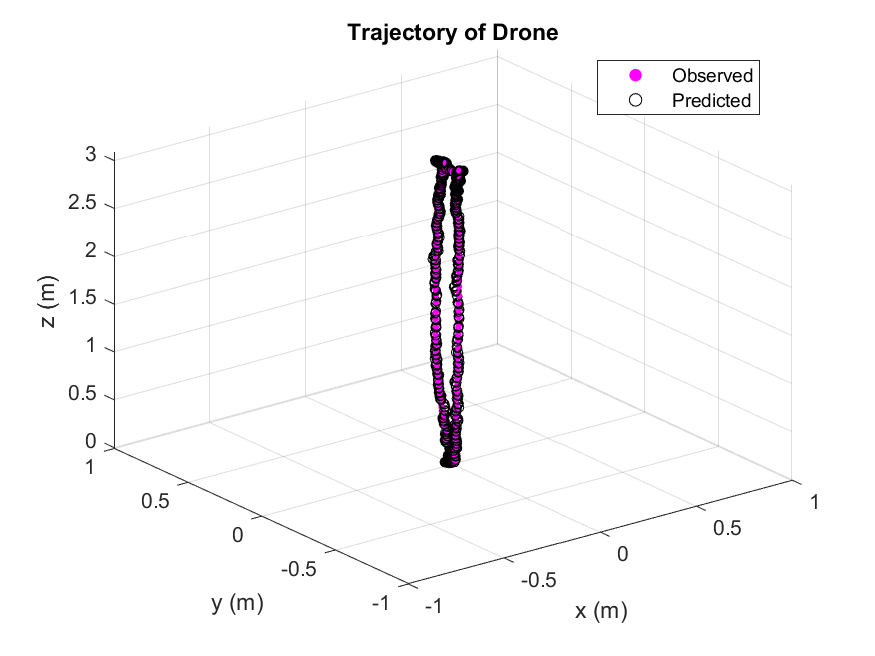
\includegraphics[width=\textwidth]{Figures/hover1_traj}
	\caption{Hover trajectory}
	\label{fig:hover1_traj}
\end{subfigure}%
\begin{subfigure}{.5\textwidth}
	\centering
	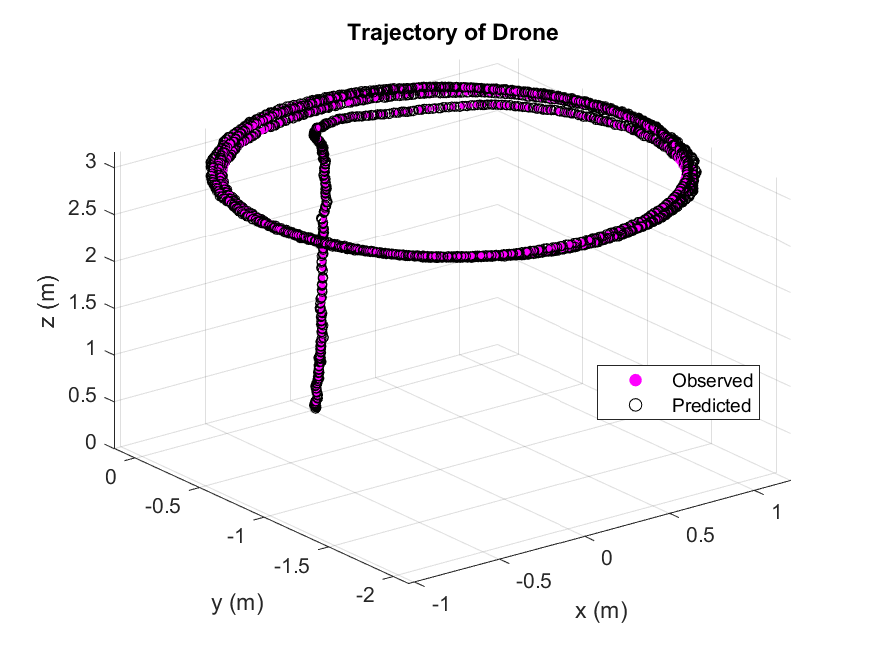
\includegraphics[width=\textwidth]{Figures/circle1_traj}
	\caption{Circle trajectory}
	\label{fig:circle1_traj}
\end{subfigure}
\caption{The observed trajectories (magenta) overlayed with the estimated drone position (black) for the hover and circle trajectories}
\label{fig:Overlay1}
\end{figure}
\begin{figure}[H]
\centering
\begin{subfigure}{.5\textwidth}
	\centering
	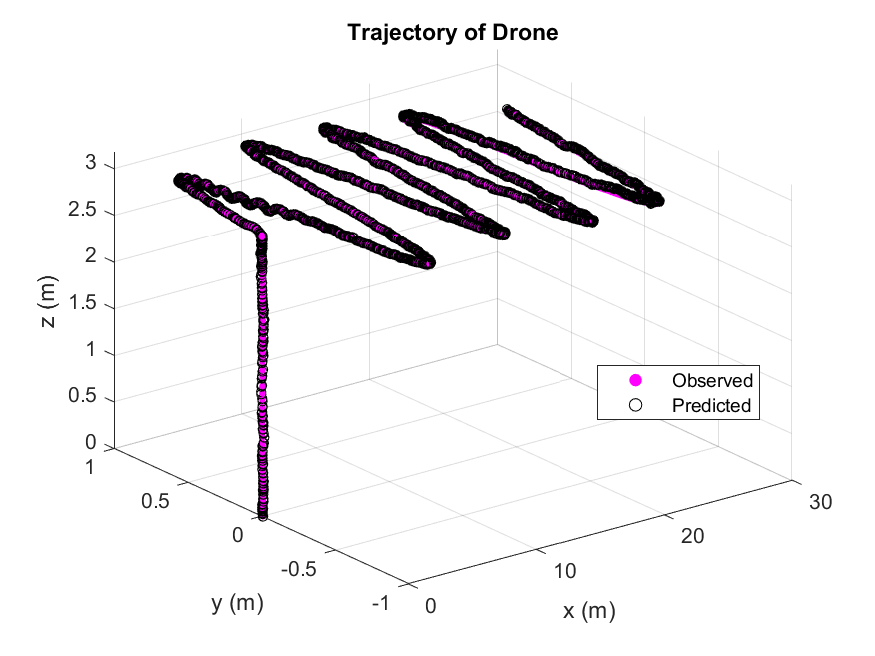
\includegraphics[width=\textwidth]{Figures/sine1_traj}
	\caption{Sine trajectory}
	\label{fig:sine1_traj}
\end{subfigure}%
\begin{subfigure}{.5\textwidth}
	\centering
	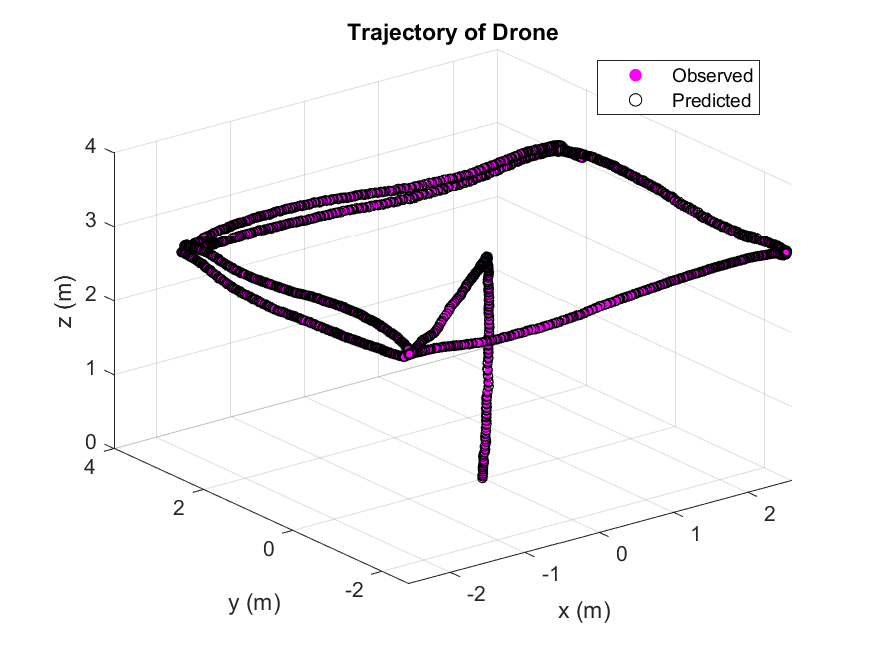
\includegraphics[width=\textwidth]{Figures/square1_traj}
	\caption{Square trajectory}
	\label{fig:square1_traj}
\end{subfigure}
\caption{The observed trajectories (magenta) overlayed with the estimated drone position (black) for the sine and square trajectories}
\label{fig:Overlay2}
\end{figure}

It can be seen from Tables~\ref{tab:sigmax} through~\ref{tab:sigmaz} that the error in actual position and estimated position increases for all trajectories as the sampling rate is decreased. This is intuitive because as the resolution of data decreases, the system has to use its knowledge of the system's dynamics to propagate itself to the next state, and this may differ from the system's observed behavior. Figures~\ref{fig:SquareErr} and \ref{fig:SquareErrTwo} show how the position error changes with time. The magnitude of error is higher when the drone maneuvers rapidly in a certain direction, and this can also be attributed to differences in the propagated state and observed state.

\begin{figure}[H]
\centering
\begin{subfigure}{.5\textwidth}
	\centering
	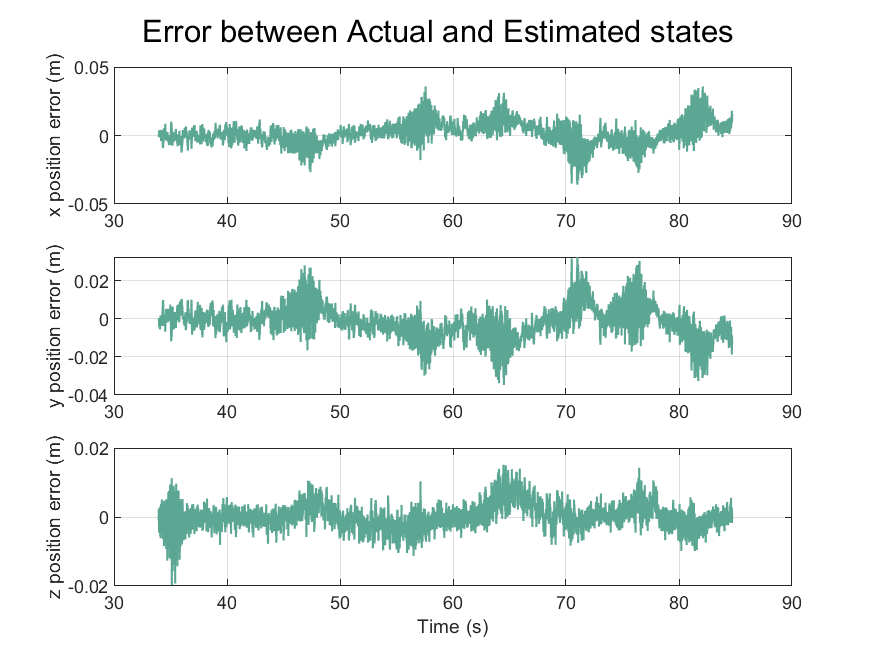
\includegraphics[width=\textwidth]{Figures/square1_err}
	\caption{Position error on the square trajectory}
	\label{fig:SquareErr1}
\end{subfigure}%
\begin{subfigure}{.5\textwidth}
	\centering
	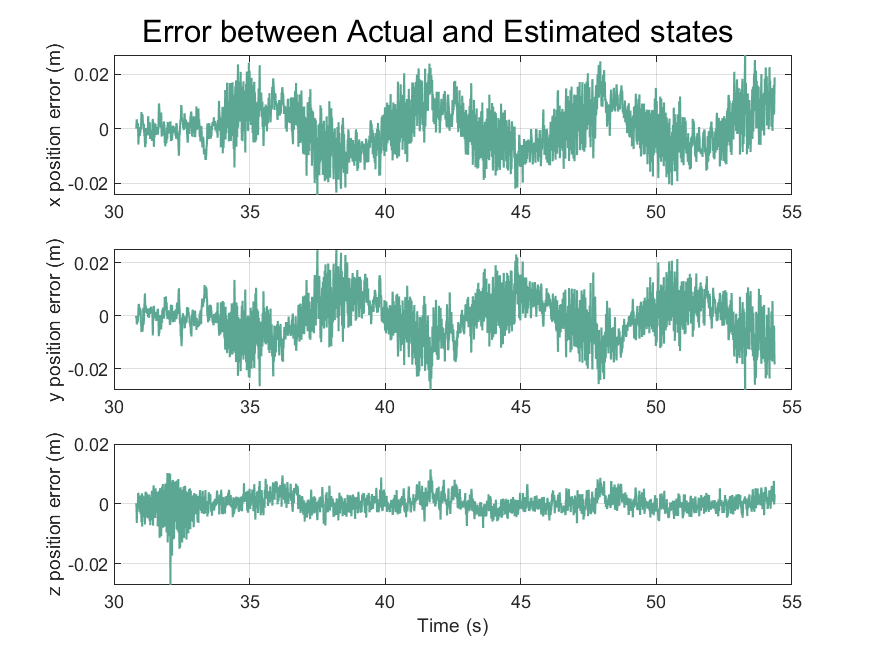
\includegraphics[width=\textwidth]{Figures/circle1_err}
	\caption{Position error on the circle trajectory}
	\label{fig:SquareErr2}
\end{subfigure}
\caption{Error between predicted and actual positions on the square and circle trajectories}
\label{fig:SquareErr}
\end{figure}
\begin{figure}[H]
\centering
\begin{subfigure}{.5\textwidth}
	\centering
	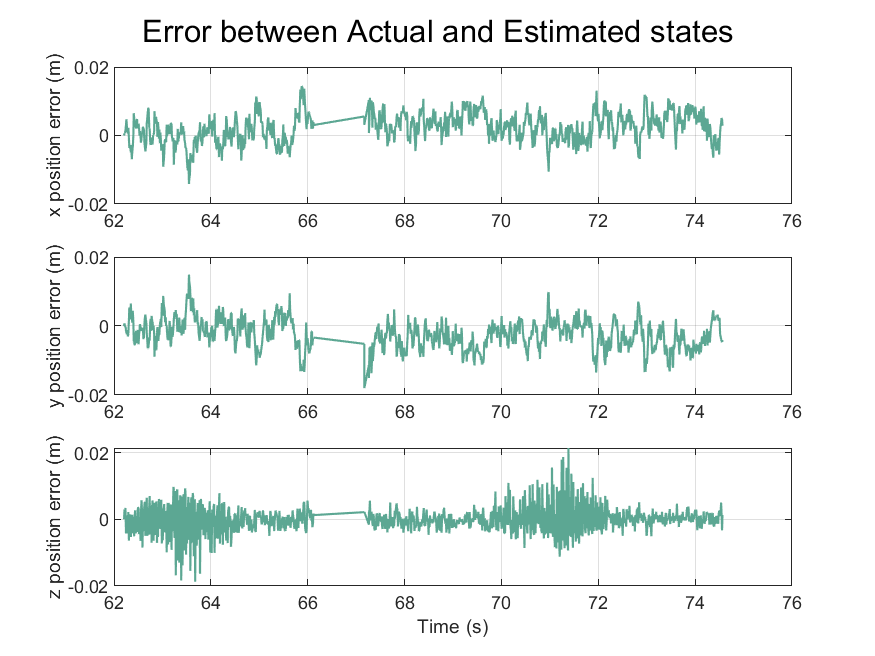
\includegraphics[width=\textwidth]{Figures/hover1_err}
	\caption{Position error on the hover trajectory}
	\label{fig:SquareErr5}
\end{subfigure}%
\begin{subfigure}{.5\textwidth}
	\centering
	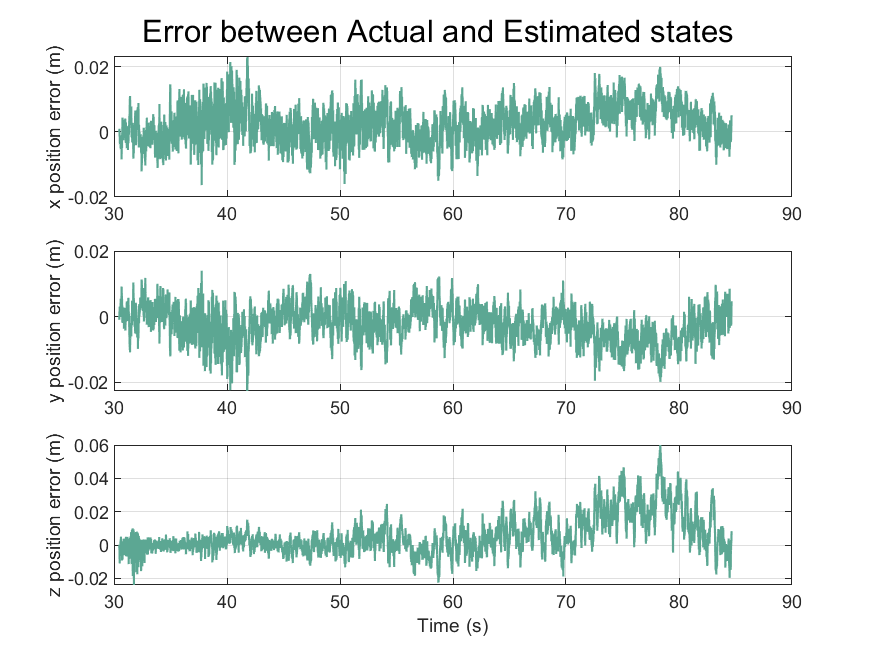
\includegraphics[width=\textwidth]{Figures/sine1_err}
	\caption{Position error on the sine trajectory}
	\label{fig:SquareErr10}
\end{subfigure}
\caption{Error between predicted and actual positions on the hover and sine trajectories}
\label{fig:SquareErrTwo}
\end{figure}



That being said, Figures~\ref{fig:SquareErr} and \ref{fig:SquareErrTwo} show that the filter is still accurate to a hundredth of a meter, and having centimeter-level accuracy is incredible when considering that the errors in the measurements from the motion capture cameras were greatly exaggerated (i.e. $1.5$ mm, $1.5$ cm, $2$ mm, and $10$ cm of error was respectively simulated in each of the four cameras instead of the rated values of $1.5$ mm\cite{V16}). %It can also be noticed that the error along a certain direction peaks when the drone is at the ends of the trajectory in that direction. This is due to the fact that the highest difference between the observed state and the state according to the dynamics occurs at the extremes of the trajectory. This can be improved with better tuning of the $Q$ matrix, as that will force the filter to prioritize the measurements.

The results of the Unscented Kalman Filter will be discussed next. The first noticeable difference between the EKF and UKF was their runtime. Table~\ref{tab:RunTime} shows the runtimes of the EKF and UKF (measured using MATLAB's \texttt{tic} and \texttt{toc} functions) for different trajectories. The UKF takes 24 times longer per iteration than the EKF, mainly due to generating and propagating sigma points. With an average runtime of 2.9589 seconds, it is not a viable option to put the UKF on an embedded system to control a drone.

\begin{table}[H]
\centering
\caption{Runtimes (in seconds) of the EKF and UKF over all trajectories at a sample rate of 6 Hz}
\label{tab:RunTime}
\begin{tabular}{|r|l|l|}
\hline
\multicolumn{1}{|l|}{\backslashbox{Trajectory}{Filter}} & \multicolumn{1}{c|}{EKF} & UKF             \\ \hline
Hover                                                   & 0.125                    & 2.8026          \\
Circle                                                  & 0.12666                  & 3.0158          \\
Square                                                  & 0.11342                  & 2.9119          \\
Sine                                                    & 0.12442                  & 3.0153          \\ \hline
\textbf{Average}                                        & \textbf{0.12238}         & \textbf{2.9589} \\ \hline
\end{tabular}
\end{table}

\begin{figure}[H]
\centering
\begin{subfigure}{.5\textwidth}
	\centering
	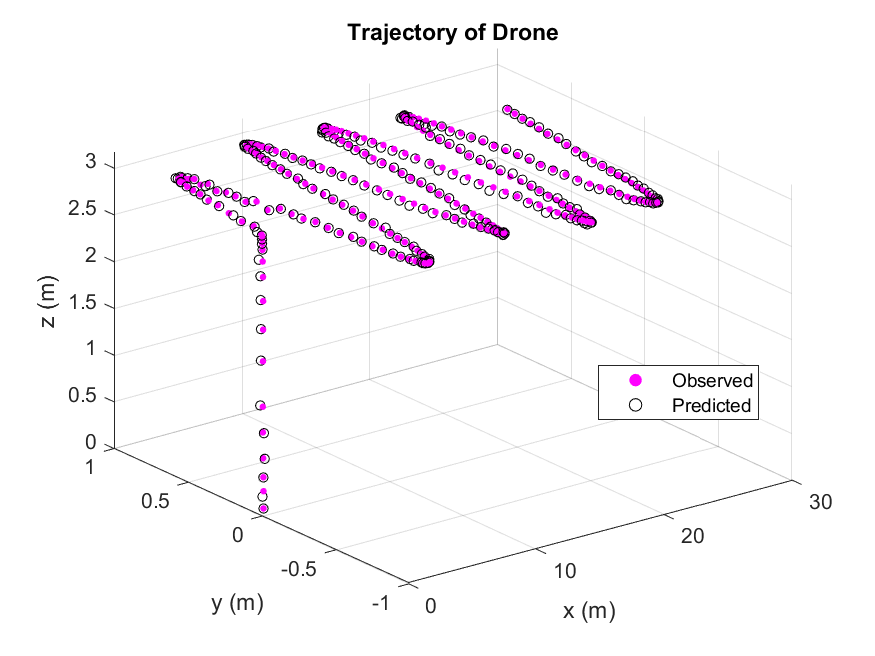
\includegraphics[width=\textwidth]{Figures/sine20_traj_UKF}
	\caption{UKF position estimates on the sine trajectory}
	\label{fig:SineUKF}
\end{subfigure}%
\begin{subfigure}{.5\textwidth}
	\centering
	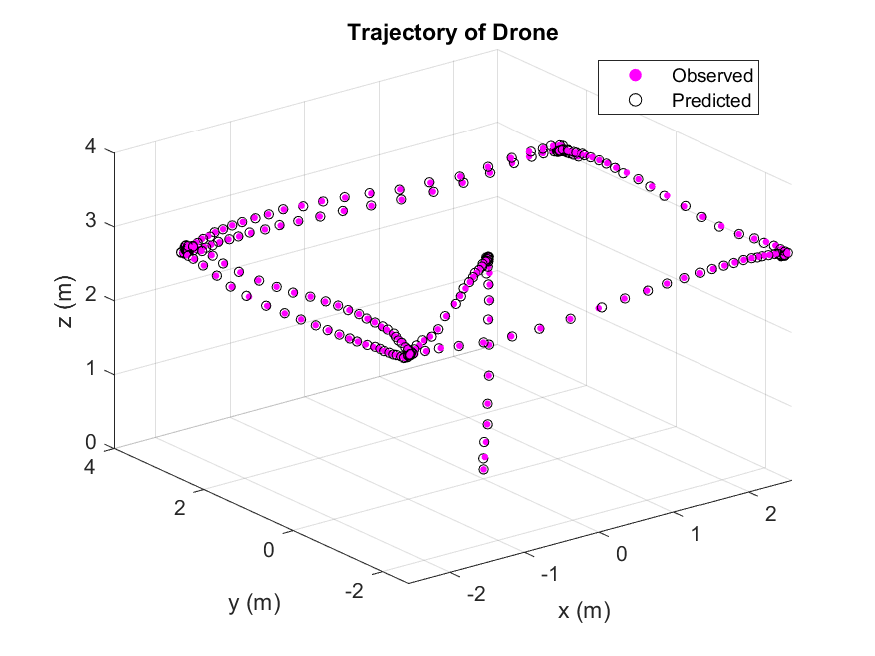
\includegraphics[width=\textwidth]{Figures/square20_traj_UKF}
	\caption{UKF position estimates on the square trajectory}
	\label{fig:SquareErr2}
\end{subfigure}
\caption{UKF position estimates on the sine trajectory at a sample rate of 6 Hz(only two trajectories were shown to save space)}
\label{fig:UKF}
\end{figure}

Figure~\ref{fig:UKF} shows the position estimates from the UKF, and Table~\ref{tab:UKFsigma} shows the standard deviation of the position error of the UKF estimates. When compared with the ``6 Hz'' row of Tables~\ref{tab:sigmax} through~\ref{tab:sigmaz}, it can be seen that the UKF estimates are slightly better, with an improvement of approximately 2 mm. This slight improvement in accuracy does not outweigh the UKF's massive increase in runtime, especially considering that the filter will need to be deployed on an embedded system to control the drone.

\begin{table}[H]
\centering
\caption{Standard deviation of the position error of UKF estimates at a sample rate of 6 Hz}
\label{tab:UKFsigma}
\begin{tabular}{|r|l|l|l|l|}
\hline
\multicolumn{1}{|l|}{\backslashbox{Direction}{Trajectory}} & \multicolumn{1}{c|}{Hover} & \multicolumn{1}{c|}{Circle} & \multicolumn{1}{c|}{Square} & \multicolumn{1}{c|}{Sine} \\ \hline
$\sigma_x$                                                 & 0.013826                   & 0.010209                    & 0.0094935                   & 0.0099276                 \\
$\sigma_y$                                                 & 0.015173                   & 0.010124                    & 0.0094954                   & 0.0095272                 \\
$\sigma_z$                                                 & 0.0049896                  & 0.0057478                   & 0.0043911                   & 0.01642                   \\ \hline
\textbf{Average}                                           & \textbf{0.01133}           & \textbf{0.008694}           & \textbf{0.010209}           & \textbf{0.011958}         \\ \hline
\end{tabular}
\end{table}

Now that it has been verified that the EKF is a better option for the application that is being studied, the EKF will be rerun with measurement error values that are more consistent with the real-life specifications of the motion capture cameras. Recall that the variances of the cameras were greatly exaggerated for this study. According to the Vicon Vantage V16's specsheet \cite{V16}, the cameras have an error of 1.5 mm. After changing the $R$ matrix to reflect this, the errors of the EKF change as can be seen graphically in Figure~\ref{fig:NewSigma} or numerically in Table~\ref{tab:NewSigma}. Unsurprisingly, the standard deviations of the position errors are much better when compared to the errors with the perturbed $R$ matrix.

\begin{figure}[H]
	\centering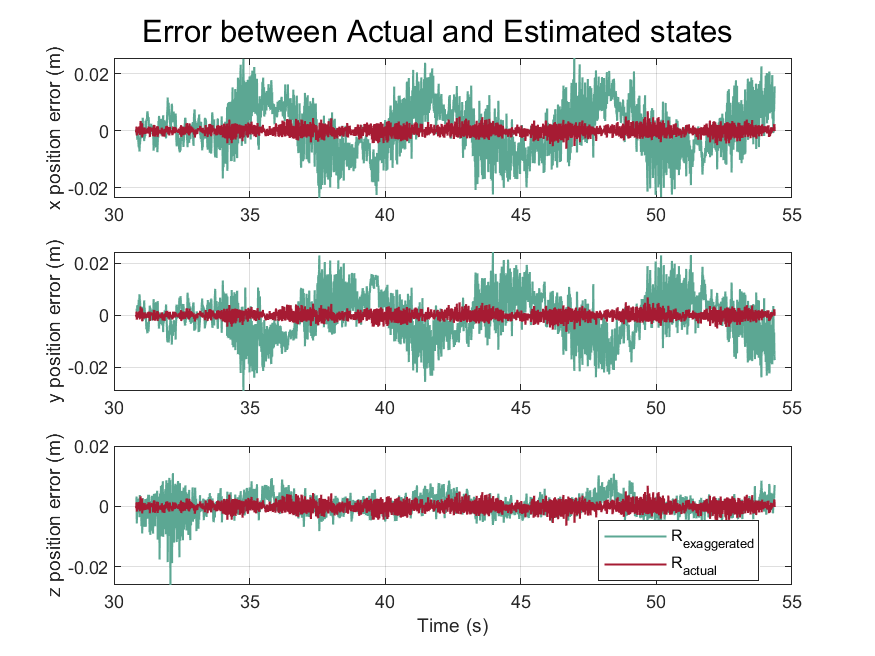
\includegraphics[width=0.8\textwidth]{Figures/_BAK_err}
	\caption{Comparison of the position error when using the actual errors ($R_a=R_{actual}$) v.s. the exaggerated errors ($R_{e}=R_{exaggerated}$)}
	\label{fig:NewSigma}
\end{figure}

% Please add the following required packages to your document preamble:
% \usepackage{multirow}
\begin{table}[H]
\centering
\caption{Standard deviation of the position error when using the actual errors ($R_a=R_{actual}$) v.s. the exaggerated errors ($R_{e}=R_{exaggerated}$)}
\label{tab:NewSigma}
\begin{tabular}{|r|ll|ll|}
\hline
\multirow{2}{*}{\ } & \multicolumn{2}{c|}{Hover} & \multicolumn{2}{c|}{Circle} \\ \cline{2-5} 
 & \multicolumn{1}{c|}{$R_{a}$} & \multicolumn{1}{c|}{$R_{e}$} & \multicolumn{1}{c|}{$R_{a}$} & \multicolumn{1}{c|}{$R_{e}$} \\ \hline
$\sigma_x$ & \multicolumn{1}{l|}{0.0010586} & 0.0042149 & \multicolumn{1}{l|}{0.0016466} & 0.0084198 \\ \hline
$\sigma_y$ & \multicolumn{1}{l|}{0.0012544} & 0.0042601 & \multicolumn{1}{l|}{0.0016962} & 0.0083595 \\ \hline
$\sigma_z$ & \multicolumn{1}{l|}{0.0023459} & 0.0038442 & \multicolumn{1}{l|}{0.0017194} & 0.0030611 \\ \hline
\end{tabular}
\end{table}

% Please add the following required packages to your document preamble:
% \usepackage{multirow}
\begin{table}[H]
\centering
\begin{tabular}{|r|ll|ll|}
\hline
\multirow{2}{*}{\ } & \multicolumn{2}{c|}{Square} & \multicolumn{2}{c|}{Sine} \\ \cline{2-5} 
 & \multicolumn{1}{c|}{$R_{a}$} & \multicolumn{1}{c|}{$R_{e}$} & \multicolumn{1}{c|}{$R_{a}$} & \multicolumn{1}{c|}{$R_{e}$} \\ \hline
$\sigma_x$ & \multicolumn{1}{l|}{0.0015686} & 0.0083749 & \multicolumn{1}{l|}{0.0014993} & 0.0054409 \\ \hline
$\sigma_y$ & \multicolumn{1}{l|}{0.0015528} & 0.0083918 & \multicolumn{1}{l|}{0.0012982} & 0.0052932 \\ \hline
$\sigma_z$ & \multicolumn{1}{l|}{0.0015894} & 0.003646 & \multicolumn{1}{l|}{0.0022801} & 0.011294 \\ \hline
\end{tabular}
\end{table}

\section{Conclusion}

In this study, a hybrid Extended Kalman filter and an Unscented Kalman filter were implemented on the dynamics of a drone. In order to improve the quality of the study, an LQR controller was used to determine the inputs to the system at each timestep, thereby increasing the types of trajectories that could be analyzed, as opposed to past studies that just involved the drone hovering or with constant inputs. Simulated measurements from Gazebo were used to test the filter. Through this study, it was noted that even with greatly exaggerated measurement covariances, the EKF was able to predict the position of the drone with centimeter-level accuracy. When the measurement covariances were changed to more closely reflect their actual values, the filter performed exceptionally well, showing millimeter-level accuracy. It was also noted that the UKF provided a slight improvement in accuracy, but took 24 times longer than the EKF. The slight improvement in accuracy does not outweigh the massive increase in runtime, and hence it can be concluded that implementing the UKF on an embedded system is not a viable option. This study proved that the EKF is accurate, quick, and robust to measurement perturbations.

\section{Acknowledgments}

Thanks to Dr. Brian Gunter for a great semester. I'd heard of Kalman filters through my work in the past, but I hadn't known how they functioned. I learned a lot through this class, and the way he taught the subject was very interesting, so much so that I've asked my manager to try to put me on a project involving research Kalman filters this summer. I'm looking forward to working more intricately with Kalman filters and applying what I've learned from this class. I also wanted to give a disclaimer that I produced many more plots, but didn't include a lot of them in this report, since their information was conveyed through other plots. They can be found in the addendum that will be submitted with this paper.

\bibliographystyle{AAS_publication}   % Number the references.
%\bibliography{references}   % Use references.bib to resolve the labels.
\begin{thebibliography}{10}

\bibitem{iris}
``3DR iris - the ready to fly UAV Quadcopter,'' Arduino based Arducopter UAV, the open source multi-rotor. \url{http://www.arducopter.co.uk/iris-quadcopter-uav.html}

\bibitem{ViconMotionCaptureSpace}
10-camera Vicon Motion Capture System. University of Saskatchewan. \url{https://research-groups.usask.ca/ergolab/our-lab.php#LabbasedEquipment}

\bibitem{LQRBook}
  Anderson, B. D. O., \& Moore, J. B. (2007). Optimal control: Linear quadratic methods. Courier Corporation.

\bibitem{DroneFrame}
Arroyo, R. (2017). A Multi-Sensorial Simultaneous Localization and Mapping (SLAM) System for Low-Cost Micro Aerial Vehicles in GPS-Denied Environments - Scientific Figure on ResearchGate. Available from: \url{https://www.researchgate.net/figure/Coordinate-frames-D-S-and-W-drone-frame-D-is-attached-to-the-drones-body_fig1_316927341} [accessed 27 Apr, 2022]

\bibitem{Alejandro}
Colina-Valeri, A. (2021). The Need for Kalman Filter to Estimate a Drones Sensor Data. In \url{https://sites.tufts.edu/eeseniordesignhandbook/files/2021/05/Colina-Valeri_KalmanFilterEstimates.pdf}.

\bibitem{gazebo}
Gazebo \url{http://gazebosim.org/}

\bibitem{X4dot}
Gibiansky, A., ``Andrew Gibiansky - Quadcopter Dynamics and Simulation,'' \url{https://andrew.gibiansky.com/blog/physics/quadcopter-dynamics/}

\bibitem{LQR}
``Linear-Quadratic Regulator (LQR) design,'', MATLAB. \url{https://www.mathworks.com/help/control/ref/lqr.html}

\bibitem{Study2}
M. Patel and P. Ferguson, ``Drone-Based Cable-Suspended Payload Tracking and Estimation Using Simulated LiDAR Measurements and an Extended Kalman Filter,'' AIAA SCITECH 2022 Forum, 2022, doi: 10.2514/6.2022-2290.

\bibitem{Study}
M. Patel and P. Ferguson, ``Tracking and Estimation of a Swaying Payload Using a LiDAR and an Extended Kalman Filter,'' 2021 IEEE International Symposium on Robotic and Sensors Environments (ROSE), 2021, pp. 1-7, doi: 10.1109/ROSE52750.2021.9611771.

\bibitem{ros}
``Robot operating system, ROS'' \url{https://www.ros.org/}

\bibitem{Simon}
Simon, D. (2006). Optimal state estimation: Kalman, H infinity, and nonlinear approaches. John Wiley \& Sons.

\bibitem{MotionCaptureDrone}
Tobias, ``Mocap Deck,'' \url{https://www.bitcraze.io/2018/06/mocap-deck/}

\bibitem{V16}
  Vantage. (2019, May 31). Vicon. \url{https://www.vicon.com/hardware/cameras/vantage/}

\bibitem{vicon_2022}
``Vicon in use: Case studies: Motion capture systems,''  Jan 2022. \url{https://www.vicon.com/resources/case-studies/the-role-of-motion-capture-in-education-is-changing-fast/}.

\end{thebibliography}


\pagebreak
\appendix
\section*{Appendix A: Algorithms}
\begin{algorithm}[H]
\footnotesize
\caption{Hybrid Extended Kalman filter\cite{Simon}}
\label{alg:EKF}
\begin{algorithmic}[1]
\State Recognize system equations $\hat{x}=f(x,u,w,t), y_k=h_k(x_k,v_k), w(t)\sim(0,Q), v_k\sim(0,R)$
\State Initialize $x_{initial}$, $P$, $Q$, $R$
\State Set $\hat{x}_{k-1}^+ \gets x_{initial}$, $P_{k-1}^+ \gets P$
\For{each measurement $y$}
    \State Assemble $y_{obs}$ by reading in measurements at $t_k$
    \State $dt \gets t_k - t_{k-1}$
    \State $\hat{x}_k^- \gets$ propagate $\hat{x}_{k-1}^+$ using the dynamics $\dot{\hat{x}}_k$ over $dt$ using ode45
    \State $A \gets$ assemble according to Eq.~\ref{eq:A}
    \State $\dot{P} \gets AP_{k-1}^+ + P_{k-1}^+A^T + Q$
    \State Assemble $y_{comp}$ according to Eq.~\ref{eq:G} using $\hat{x}_k^-$
    \State Assemble $H_k$ according to Eq.~\ref{eq:H} using $\hat{x}_k^-$ and coordinates in Table~\ref{tab:cameras}
    \State $P_k^- \gets P_{k-1}^+ + \dot{P}\times dt$
    \State $K_k \gets P_k^- H_k^T(H_kP_k^-H_k^T+R)^{-1}$
    \State $\hat{x}_k^+ \gets \hat{x}_k^- + K_k(y_{obs}-y_{comp}$
    \State $P_k^+\gets (I_{12}-K_kH_k)P_k^-(I_{12}-K_kH_k)^T + R$
\EndFor
\end{algorithmic}
\end{algorithm}


\begin{algorithm}[H]
\footnotesize
\caption{Unscented Kalman filter\cite{Simon}}
\label{alg:UKF}
\begin{algorithmic}[1]
\State Recognize system equations $x_{k+1}=f(x_k,u_k,t_k)+w_k, y_k=h(x_k,t_k)+v_k, w(t)\sim(0,Q_k), v_k\sim(0,R_k)$
\State Initialize $x_{initial}$, $P$, $Q$, $R$
\State Set $\hat{x}_{k-1}^+ \gets x_{initial}$, $P_{k-1}^+ \gets P$, $n \gets$ number of states
\For{each measurement $y$}
    \State Assemble $y_{obs}$ by reading in measurements at $t_k$
    \State $dt \gets t_k - t_{k-1}$
    \For{j=1:2n}
    		\State $\hat{x}_{k-1}^{(i)} \gets \hat{x}_{k-1}^+ + \tilde{x}^{(i)}; \quad i=1,\cdots,2n$
    		\State $\tilde{x}^{(i)} \gets (\sqrt{nP_{k-1}^+})_i^T; \quad i=1,\cdots,n$
    		\State $\tilde{x}^{(n+i)} \gets -(\sqrt{nP_{k-1}^+})_i^T; \quad i=1,\cdots,n$
    	\EndFor
    \State $\hat{x}_k^{(i)} \gets$ propagate $\hat{x}_{k-1}^{(i)}$ using the dynamics $\dot{\hat{x}}_k^{(i)}$ over $dt$ using ode45
    \State $\hat{x}_k^- \gets \frac{1}{2n}\sum_{i=1}^{2n}\hat{x}_k^{(i)}$
    \State $P_k^- \gets \frac{1}{2n}\sum_{i=1}^{2n}(\hat{x}_k^{(i)}-\hat{x}_k^-)(\hat{x}_k^{(i)}-\hat{x}_k^-)^T + Q_{k-1}$
    \For{j=1:2n}
    		\State $\hat{x}_{k}^{(i)} \gets \hat{x}_{k}^+ + \tilde{x}^{(i)}; \quad i=1,\cdots,2n$
    		\State $\tilde{x}^{(i)} \gets (\sqrt{nP_{k}^+})_i^T; \quad i=1,\cdots,n$
    		\State $\tilde{x}^{(n+i)} \gets -(\sqrt{nP_{k}^+})_i^T; \quad i=1,\cdots,n$
    	\EndFor
    \State Assemble $\hat{y}_{k}^{(i)}$ according to Eq.~\ref{eq:G} using $\hat{x}_k^{(i)}$
    \State $\hat{y}_k \gets \frac{1}{2n}\sum_{i=1}^{2n}\hat{y}_k^{(i)}$
    \State $P_y \gets \frac{1}{2n}\sum_{i=1}^{2n}(\hat{y}_k^{(i)}-\hat{y}_k)(\hat{y}_k^{(i)}-\hat{y}_k)^T + R_k$
    \State $P_{xy} \gets \frac{1}{2n}\sum_{i=1}^{2n}(\hat{x}_k^{(i)}-\hat{x}_k^-)(\hat{y}_k^{(i)}-\hat{y}_k)^T$
    \State $K_k \gets P_{xy}P_y^{-1}$
    \State $\hat{x}_k^+ \gets \hat{x}_k^- + K_k(y_{obs}-\hat{y}_k)$
    \State $P_k^+ \gets P_k^- - K_kP_yK_k^T$
\EndFor
\end{algorithmic}
\end{algorithm}

\end{document}
